\documentclass[12pt]{article}

% Core math
\usepackage{amsmath, amssymb, amsthm}

% Diagrams
\usepackage{tikz-cd}
\usepackage{tikz}

% References and links
\usepackage{hyperref}
\usepackage{cleveref}

% Graphics
\usepackage{graphicx}

% Page layout
\usepackage[margin=1in]{geometry}

% Sidebar
\usepackage{everypage}
\usepackage{xcolor}
\usepackage{booktabs}

% Theorem environments
\newtheorem{theorem}{Theorem}[section]
\newtheorem{proposition}[theorem]{Proposition}
\newtheorem{lemma}[theorem]{Lemma}
\newtheorem{corollary}[theorem]{Corollary}
\theoremstyle{definition}
\newtheorem{definition}[theorem]{Definition}
\newtheorem{example}[theorem]{Example}
\theoremstyle{remark}
\newtheorem{remark}[theorem]{Remark}
\newtheorem{hook}[theorem]{Composition Hook}

% Macros
\newcommand{\C}{\mathcal{C}}
\newcommand{\D}{\mathcal{D}}
\newcommand{\E}{\mathcal{E}}
\newcommand{\Phys}{\mathbf{Phys}}
\newcommand{\Info}{\mathbf{Info}}
\newcommand{\Hilb}{\mathbf{Hilb}}
\newcommand{\FHilb}{\mathbf{FHilb}}
\newcommand{\Vect}{\mathbf{Vect}}
\newcommand{\Set}{\mathbf{Set}}
\newcommand{\Cob}{\mathbf{Cob}}
\newcommand{\Bord}{\mathbf{Bord}}
\newcommand{\op}{\mathrm{op}}
\newcommand{\id}{\mathrm{id}}
\newcommand{\Hom}{\mathrm{Hom}}
\newcommand{\End}{\mathrm{End}}
\newcommand{\Tr}{\mathrm{Tr}}
\newcommand{\Ob}{\mathrm{Ob}}

% GrokRxiv sidebar
\definecolor{grokgray}{RGB}{110,110,110}
\AddEverypageHook{%
  \ifnum\value{page}=1
    \begin{tikzpicture}[remember picture, overlay]
      \node[
        rotate=90,
        anchor=south,
        font=\Large\sffamily\bfseries\color{grokgray},
        inner sep=0pt
      ] at ([xshift=38pt, yshift=0.52\paperheight]current page.south west)
      {GrokRxiv:2026.04.mathematical-formalisms\quad
       [\,math.CT\,]\quad
       30 Apr 2026};
    \end{tikzpicture}
  \fi
}

\title{Law I --- Mathematical Formalisms:\\
Categorical Foundations for Matter--Information Correspondence}
\author{MagnetonIO Research \\
\textit{Emergent Spacetime Dynamics Series, Paper 1 of 4}}
\date{30 April 2026}

\begin{document}
\maketitle

\begin{abstract}
We formulate the categorical grammar underlying a modular four-law programme for emergent spacetime dynamics. Law~I, presented here, is the foundational layer: it fixes the language in which Laws~II (phase-bound matter), III (frequency-modulated processes), and IV (information-bearing structures) are written. We argue that the appropriate mathematical setting for a matter--information correspondence is that of symmetric monoidal $(\infty,n)$-categories together with their sheaf-theoretic, operadic, and type-theoretic refinements. We isolate eight \emph{composition hooks}---formal interfaces marked $\mathsf{H1}$--$\mathsf{H8}$---that downstream laws plug into without modification. We define the matter--information functor $M : \Phys \to \Info$ as a strong monoidal, dagger-preserving functor between symmetric monoidal dagger categories, and we prove three structural results: (i) $M$ is fully determined on a generating set under the cobordism hypothesis; (ii) preservation of duals under $M$ implies a Born-rule-type formula on traceable processes; (iii) a sheaf condition for local observables lifts uniquely to a sheaf condition on $M$-images. We supply a Haskell encoding of the categorical core (a \texttt{Category}/\texttt{MonoidalCategory}/\texttt{Functor1} hierarchy with QuickCheck property tests), and worked examples drawn from finite-dimensional Hilbert spaces, the cobordism category, the topos of presheaves on a poset, and the little-disks operad. The paper is explicitly modular: nothing here pretends to a unified theory of physics. Rather, it provides the substrate onto which subsequent laws are functorially composed.
\end{abstract}

\tableofcontents

\section{Introduction}
\label{sec:introduction}

\subsection{Modular framework, not unified theory}

Modern theoretical physics is replete with frameworks that aspire to unification. The programme to which this paper belongs makes no such claim. We instead pursue a \emph{modular} approach: we identify a small number of mathematical layers, each of which is autonomous and self-standing, and we organise their interaction through explicit \emph{composition hooks}. The hooks are formal: they are functor signatures, sheaf conditions, or operadic action squares whose existence is asserted in Law~I and whose realisation is supplied by Laws~II, III, and IV.

This paper is Law~I. It establishes the categorical primitives that the other three laws will compose onto. Its claims are not physical in the empirical sense---no Hamiltonian, no scattering amplitude, no thermodynamic measurement appears as a primitive object. Its claims are structural: \emph{if} we accept that physical processes are arrows in some category $\Phys$, and \emph{if} we accept that informational descriptions live in some category $\Info$, then the relation between them must be a structure-preserving functor whose domain and codomain admit specific composition properties.

\subsection{Why categorical language?}

Three reasons motivate the choice. First, physical systems compose, both spatially (tensor products of subsystems) and temporally (sequential evolution); the algebra of these two compositions, together with their compatibility, is exactly what monoidal category theory was designed to formalise~\cite{maclane1998}. Second, observables organise locally and assemble globally: this is the sheaf-theoretic structure familiar from gauge theory, and its higher-categorical refinement underlies modern formulations of quantum field theory~\cite{costello2017}. Third, the same algebraic data---a symmetric monoidal closed (or compact closed) category---governs quantum mechanics, computation, logic, and topology, as exhibited in the Rosetta Stone of Baez and Stay~\cite{baezstay2009}. Taking the Rosetta Stone seriously means that the matter--information correspondence is not a physical accident but a four-way translational symmetry built into the categorical substrate.

\subsection{Composition hooks: where Laws II--IV plug in}

A central methodological device of this paper is the explicit declaration of \emph{composition hooks}. A hook is a typed slot: it specifies the categorical signature that a downstream construction must populate. We declare eight hooks:
\begin{itemize}
\item $\mathsf{H1}$ (Symmetry-action hook): a category of symmetry data $\mathcal{G}$ acting on $\Phys$ via a functor $\rho: B\mathcal{G} \to \mathrm{Aut}(\Phys)$. Used by Law~II to encode global symmetries of phases of matter.
\item $\mathsf{H2}$ (Hamiltonian hook): a designated subcategory $\mathbf{Ham} \hookrightarrow \Phys$ closed under tensor product. Used by Laws~II, III to define gapped Hamiltonians and adiabatic deformations.
\item $\mathsf{H3}$ (Floquet hook): a circle category $B\mathbb{Z}$ and an action $B\mathbb{Z} \to \mathrm{Aut}(\Phys)$. Used by Law~III to encode periodic drive.
\item $\mathsf{H4}$ (Sheaf hook): a Grothendieck site $(\C, J)$ controlling locality of observables. Used by Law~II to handle local order parameters and by Law~IV for boundary CFT data.
\item $\mathsf{H5}$ (Operadic hook): an operad $O$ acting on a designated object of $\Info$. Used by Law~IV for factorisation algebras.
\item $\mathsf{H6}$ (Dagger hook): the dagger structure $\dagger$ on $\Phys$ and its preservation by $M$. Used by Law~III for unitary drive operators.
\item $\mathsf{H7}$ (Compact-closure hook): existence of duals in $\Phys$ and $\Info$. Used by Law~IV for traces, partial traces, and the Ryu--Takayanagi formula.
\item $\mathsf{H8}$ (Type-theoretic hook): an internal language $\mathcal{L}(\Info)$ obtained from a topos structure. Used by all subsequent laws for executable encoding.
\end{itemize}

We mark these hooks throughout the text. They are the contract between Law~I and the remainder of the series.

\subsection{Outline}

\Cref{sec:preliminaries} reviews categorical preliminaries with the precision needed for the sequel. \Cref{sec:matter-info-functor} introduces the matter--information functor $M$ and proves its basic structural properties. \Cref{sec:monoidal} develops the monoidal structure of state spaces. \Cref{sec:sheaves} formalises sheaves and topoi for local physics. \Cref{sec:operads} treats operadic composition. \Cref{sec:type-theory} gives the type-theoretic encoding. \Cref{sec:examples} works concrete examples. \Cref{sec:open-problems} states open problems for Law~I as a foundational layer. \Cref{sec:conclusion} closes.

\section{Categorical Preliminaries}
\label{sec:preliminaries}

We fix conventions. Throughout, ``category'' means a locally small category in the sense of~\cite{maclane1998}. We follow the conventions of~\cite{lurie2009} when the discussion turns to $(\infty,n)$-categories.

\subsection{Categories, functors, natural transformations}

\begin{definition}[Category]
\label{def:category}
A \emph{category} $\C$ consists of:
\begin{enumerate}
\item a class $\Ob(\C)$ of \emph{objects};
\item for every pair $A, B \in \Ob(\C)$, a set $\Hom_\C(A,B)$ of \emph{morphisms};
\item for every triple $A, B, C$, a \emph{composition} $\circ : \Hom_\C(B,C) \times \Hom_\C(A,B) \to \Hom_\C(A,C)$;
\item for every $A$, an \emph{identity} $\id_A \in \Hom_\C(A,A)$;
\end{enumerate}
satisfying associativity $(h \circ g) \circ f = h \circ (g \circ f)$ and unitality $\id \circ f = f = f \circ \id$.
\end{definition}

\begin{definition}[Functor]
A \emph{functor} $F : \C \to \D$ assigns to each $A \in \Ob(\C)$ an object $F(A) \in \Ob(\D)$ and to each morphism $f : A \to B$ a morphism $F(f) : F(A) \to F(B)$, satisfying $F(\id_A) = \id_{F(A)}$ and $F(g \circ f) = F(g) \circ F(f)$.
\end{definition}

\begin{definition}[Natural transformation]
Given functors $F, G : \C \to \D$, a \emph{natural transformation} $\eta : F \Rightarrow G$ is a family of morphisms $\eta_A : F(A) \to G(A)$, indexed by $A \in \Ob(\C)$, such that for every $f : A \to B$ in $\C$ the square
\[
\begin{tikzcd}
F(A) \arrow[r,"F(f)"] \arrow[d,"\eta_A"'] & F(B) \arrow[d,"\eta_B"] \\
G(A) \arrow[r,"G(f)"'] & G(B)
\end{tikzcd}
\]
commutes.
\end{definition}

The slogan, due to Lawvere~\cite{lawvere1963}, is that mathematics is naturally organised by adjunctions, and the present paper takes this slogan as a working principle.

\subsection{Monoidal categories}

\begin{definition}[Monoidal category]
\label{def:monoidal}
A \emph{monoidal category} is a tuple $(\C, \otimes, I, \alpha, \lambda, \rho)$ where $\C$ is a category, $\otimes : \C \times \C \to \C$ is a bifunctor, $I \in \Ob(\C)$ is a distinguished \emph{unit}, and $\alpha, \lambda, \rho$ are natural isomorphisms
\[
\alpha_{A,B,C} : (A \otimes B) \otimes C \xrightarrow{\sim} A \otimes (B \otimes C),
\quad \lambda_A : I \otimes A \xrightarrow{\sim} A,
\quad \rho_A : A \otimes I \xrightarrow{\sim} A,
\]
satisfying Mac Lane's pentagon and triangle axioms~\cite{maclane1998}.
\end{definition}

\begin{definition}[Symmetric monoidal category]
A monoidal category $(\C, \otimes, I)$ is \emph{symmetric} if equipped with a natural isomorphism $\sigma_{A,B} : A \otimes B \xrightarrow{\sim} B \otimes A$ such that $\sigma_{B,A} \circ \sigma_{A,B} = \id_{A \otimes B}$ and the symmetry hexagon commutes.
\end{definition}

\begin{theorem}[Mac Lane Coherence~\cite{maclane1998}]
\label{thm:maclane}
In any monoidal category, every diagram constructed from the structural isomorphisms $\alpha, \lambda, \rho$ commutes. Equivalently, the free monoidal category on one generator is equivalent (as a monoidal category) to the discrete category whose objects are bracketed words modulo associativity and unit, and whose only morphisms are identities.
\end{theorem}

\begin{proof}[Proof sketch]
Apply Mac Lane's strictification: every monoidal category is monoidally equivalent to a strict monoidal category, in which the structural isomorphisms are identities. The pentagon and triangle axioms suffice to ensure the strictification is well-defined.
\end{proof}

\Cref{thm:maclane} licenses our subsequent suppression of associators and unitors when no confusion arises.

\subsection{Compact closed and dagger structures}

\begin{definition}[Compact closed category]
\label{def:compact-closed}
A symmetric monoidal category $\C$ is \emph{compact closed} if every object $A$ has a \emph{dual} $A^*$ together with morphisms
\[
\eta_A : I \to A^* \otimes A,
\qquad
\varepsilon_A : A \otimes A^* \to I,
\]
called \emph{unit} and \emph{counit}, satisfying the triangle (or ``zig-zag'') identities:
\[
(\id_A \otimes \varepsilon_A) \circ (\eta_A \otimes \id_A) = \id_A,
\qquad
(\varepsilon_A \otimes \id_{A^*}) \circ (\id_{A^*} \otimes \eta_A) = \id_{A^*}.
\]
Diagrammatically (string-diagram calculus, anticipated from \cref{thm:joyal-street}), the first identity says that an $A$-strand (oriented upward) which is bent through a cup ($\eta_A$) and back through a cap ($\varepsilon_A$) ``snakes'' into a straight $A$-strand:
\[
\begin{tikzcd}[column sep=tiny, row sep=tiny]
{}\arrow[d, no head] & {} & {}\\
A \arrow[d, bend left=90, looseness=2, no head] & A^* \arrow[d, bend right=90, looseness=2, no head] & {}\\
{} & {} & A \arrow[d, no head]\\
{} & {} & {}
\end{tikzcd}
\;\;=\;\;
\begin{tikzcd}[column sep=tiny, row sep=tiny]
A \arrow[d, no head]\\
{}\\
A
\end{tikzcd}
\]
The second identity is the mirror image with $A$ and $A^*$ exchanged.
\end{definition}

\begin{definition}[Dagger category]
A \emph{dagger category} is a category $\C$ equipped with a contravariant involutive identity-on-objects functor $\dagger : \C^\op \to \C$ such that $(f^\dagger)^\dagger = f$. A \emph{dagger compact closed category} is a compact closed category whose dagger is compatible with the duals via $\varepsilon_A^\dagger = \sigma_{A^*,A} \circ \eta_A$~\cite{abramskycoecke2004}.
\end{definition}

\begin{example}[$\FHilb$]
\label{ex:fhilb}
Finite-dimensional complex Hilbert spaces with linear maps form a dagger compact closed symmetric monoidal category. The tensor is the Hilbert tensor product, the unit is $\mathbb{C}$, the dual of $H$ is the conjugate space $H^*$, $\eta : \mathbb{C} \to H^* \otimes H$ is $1 \mapsto \sum_i \bar{e}_i \otimes e_i$ for any basis $\{e_i\}$, $\varepsilon$ is the evaluation pairing, and $\dagger$ is the Hilbert-space adjoint~\cite{abramskycoecke2004}.
\end{example}

\subsection{The cobordism category}

\begin{definition}[$\Cob_n$]
\label{def:cob-n}
The category $\Cob_n$ has as objects closed oriented $(n-1)$-manifolds. A morphism $\Sigma_0 \to \Sigma_1$ is a diffeomorphism class of compact oriented $n$-manifolds $M$ together with an orientation-preserving diffeomorphism $\partial M \cong \overline{\Sigma_0} \sqcup \Sigma_1$. Composition is gluing along the boundary; the tensor is disjoint union; the unit is the empty $(n-1)$-manifold.
\end{definition}

$\Cob_n$ is symmetric monoidal and compact closed; the dual of $\Sigma$ is $\overline{\Sigma}$ (orientation reversal).

\begin{definition}[TQFT~\cite{atiyah1988}]
An $n$-dimensional TQFT is a symmetric monoidal functor $Z : \Cob_n \to \Vect_k$ (or $\FHilb$).
\end{definition}

\begin{theorem}[Cobordism Hypothesis~\cite{baezdolan1995,lurie2009}]
\label{thm:cobordism}
Let $\Bord_n^{\mathrm{fr}}$ denote the $(\infty,n)$-category of framed bordisms. For any symmetric monoidal $(\infty,n)$-category $\C$, the evaluation-at-the-point functor
\[
\mathrm{Fun}^{\otimes}(\Bord_n^{\mathrm{fr}}, \C) \xrightarrow{\sim} \C^{\mathrm{fd}}
\]
is an equivalence, where $\C^{\mathrm{fd}}$ is the $\infty$-groupoid of fully dualisable objects of $\C$.
\end{theorem}

We use the cobordism hypothesis as a representability principle: physical functors are determined by where they send the point, provided we work in a setting with enough duals.

\section{The Matter--Information Functor}
\label{sec:matter-info-functor}

The central object of Law~I is a structure-preserving functor $M : \Phys \to \Info$. We now define its domain, codomain, and structural conditions.

\subsection{The categories \texorpdfstring{$\Phys$}{Phys} and \texorpdfstring{$\Info$}{Info}}

\begin{definition}[$\Phys$]
\label{def:phys}
The category $\Phys$ is a symmetric monoidal dagger category whose objects are \emph{physical systems}, abstractly characterised. Morphisms are \emph{processes}: arbitrary linear, completely positive, or unitary maps depending on context. The tensor product is composition of independent systems; $\dagger$ encodes time-reversal/adjoint; $I$ is the trivial system.
\end{definition}

\begin{definition}[$\Info$]
The category $\Info$ is a symmetric monoidal dagger category whose objects are \emph{information-theoretic resources}. Examples include: classical or quantum information types; presheaves on a poset of measurement contexts; or sections of a sheaf of state spaces. Morphisms are information-preserving (or information-monotone) processes.
\end{definition}

\begin{remark}
We do not commit to a single concrete realisation of $\Phys$ or $\Info$. Different choices give different instantiations of Law~I; what is universal is the \emph{type} of the functor $M$ and the structural properties it must preserve.
\end{remark}

\subsection{Definition of \texorpdfstring{$M$}{M}}

\begin{definition}[Matter--information functor]
\label{def:matter-info}
A \emph{matter--information functor} is a strong monoidal dagger functor $M : \Phys \to \Info$. That is, $M$ is a functor equipped with natural isomorphisms
\[
\mu_{A,B} : M(A) \otimes M(B) \xrightarrow{\sim} M(A \otimes B),
\qquad
\iota : I_{\Info} \xrightarrow{\sim} M(I_{\Phys}),
\]
satisfying the standard monoidal coherence diagrams~\cite{maclane1998}, and additionally $M(f^\dagger) = M(f)^\dagger$ for every morphism $f$.
\end{definition}

\begin{hook}[Symmetry-action hook $\mathsf{H1}$]
\label{hook:H1}
Given a group $G$ with delooping $BG$, a \emph{symmetry action on $\Phys$} is a strong monoidal functor $\rho : BG \to \mathrm{Aut}_\otimes(\Phys)$. We do not require $M$ to be invertible. Instead, we say that $M$ \emph{transports} $\rho$ to an action $\rho_M : BG \to \mathrm{Aut}_\otimes(\Info)$ if for every $g \in G$ the diagram
\[
\begin{tikzcd}
\Phys \arrow[r, "\rho(g)"] \arrow[d, "M"'] & \Phys \arrow[d, "M"] \\
\Info \arrow[r, "\rho_M(g)"'] & \Info
\end{tikzcd}
\]
commutes (strictly, or up to natural isomorphism in a 2-categorical setting). When $M$ is fully faithful, such a $\rho_M$ exists and is unique on the essential image of $M$, by the universal property of the image factorisation. When $M$ is not fully faithful, the existence of a compatible transported action $\rho_M$ is no longer automatic: distinct $g \in G$ may act identically on the essential image of $M$, or the chosen symmetry of $\Phys$ may fail to descend to a well-defined action on $\Info$ at all. Law~II therefore imposes this transportability as a hypothesis: in the setting of Law~II's phase classifier, the chosen symmetry of $\Phys$ must \emph{transport} cleanly through $M$ to a compatible action on $\Info$, and the existence of such a compatible $\rho_M$ is part of the definition of a symmetric phase.
\end{hook}

This hook is what Law~II uses to encode global symmetries.

\subsection{Determination of \texorpdfstring{$M$}{M} on generators}

The cobordism hypothesis allows us to characterise $M$ on a generating subcategory.

\begin{theorem}[Generation theorem for $M$]
\label{thm:generation}
Suppose $\Phys$ is presented as a free symmetric monoidal category on a set of generating objects $\{X_i\}_{i \in I}$ and generating morphisms $\{f_j : A_j \to B_j\}_{j \in J}$, modulo a set of relations $R$. Then a strong monoidal functor $M : \Phys \to \Info$ is uniquely determined by the assignments
\[
M(X_i) \in \Ob(\Info),
\qquad
M(f_j) : M(A_j) \to M(B_j),
\]
provided the assignments respect the relations $R$, in the sense that both sides of each relation map to equal morphisms in $\Info$.
\end{theorem}

\begin{proof}
We invoke the universal property of the free symmetric monoidal category on a signature with relations.

\emph{Step 1 (Existence).} The free symmetric monoidal category $\mathrm{F}(\{X_i\}, \{f_j\})$ on the generating data, before quotienting by $R$, is constructed by taking objects to be finite formal tensor expressions in the $X_i$ (modulo the strict-monoidal coherence) and morphisms to be equivalence classes of formal expressions built from the $f_j$, identities, structural symmetries, and the operations $\circ$ and $\otimes$, modulo the bifunctoriality of $\otimes$ and the symmetric monoidal coherence laws. The data of $M$ on generators extends uniquely to a strong monoidal functor on $\mathrm{F}(\{X_i\}, \{f_j\})$ by induction on the formal expression: tensor products are mapped via the coherence isomorphisms $\mu$, compositions are mapped by composition, identities by identities, and symmetries by the symmetries of $\Info$.

\emph{Step 2 (Descent through relations).} The presentation $\Phys = \mathrm{F}(\{X_i\}, \{f_j\}) / R$ identifies certain pairs of formal expressions. The hypothesis that ``the assignments respect $R$'' means that for each relation $r = (e_1 \sim e_2) \in R$, the images $M(e_1)$ and $M(e_2)$ are equal in $\Info$. The functor $\widetilde{M} : \mathrm{F}(\{X_i\}, \{f_j\}) \to \Info$ therefore descends through the quotient to a unique functor $M : \Phys \to \Info$.

\emph{Step 3 (Uniqueness).} Any strong monoidal functor $M' : \Phys \to \Info$ agreeing with $M$ on the generators must, by the same induction, agree with $M$ on all formal expressions, hence on all morphisms. Uniqueness follows.
\end{proof}

\begin{corollary}[$M$ on the cobordism category]
\label{cor:M-on-cob}
If $\Phys = \Bord_n^{\mathrm{fr}}$, then $M$ is determined by the image of the point under $M$, provided this image is a fully dualisable object of $\Info$.
\end{corollary}

\begin{proof}
Combine \cref{thm:generation} with \cref{thm:cobordism}.
\end{proof}

\subsection{Born-rule type formula}

\begin{theorem}[Born rule from compact closure]
\label{thm:born}
Let $M : \Phys \to \Info$ be a dagger compact-preserving strong monoidal functor between dagger compact closed categories. For any state $\psi : I \to A$ in $\Phys$ and any effect $m : A \to I$, the squared norm
\[
\|m \circ \psi\|^2 := (m \circ \psi)^\dagger \circ (m \circ \psi) : I \to I
\]
is preserved by $M$ in the sense that $M(\|m \circ \psi\|^2) = \|M(m) \circ M(\psi)\|^2$.
\end{theorem}

\begin{proof}
Since $M$ is a dagger functor, $M((m \circ \psi)^\dagger) = M(m \circ \psi)^\dagger$. Since $M$ is functorial, $M(m \circ \psi) = M(m) \circ M(\psi)$. Composition then gives the claim:
\[
M(\|m \circ \psi\|^2) = M((m \circ \psi)^\dagger \circ (m \circ \psi)) = M(m \circ \psi)^\dagger \circ M(m \circ \psi) = \|M(m) \circ M(\psi)\|^2. \qedhere
\]
\end{proof}

In $\FHilb$, $\End(I) = \End(\mathbb{C}) = \mathbb{C}$, and $\|m \circ \psi\|^2 \in \mathbb{R}_{\geq 0}$ is the Born probability $|\langle m \mid \psi\rangle|^2$. \Cref{thm:born} says this number is invariant under $M$.

\begin{hook}[Compact-closure hook $\mathsf{H7}$]
\label{hook:H7}
A compact-closed structure on $\Phys$ and $\Info$, preserved by $M$, supplies the trace and partial trace operations used by Law~IV's holographic codes. Specifically, the trace $\Tr_A : \End(A) \to \End(I)$ defined by $\Tr_A(f) := \varepsilon_A \circ \sigma_{A,A^*} \circ (f \otimes \id_{A^*}) \circ \eta_A$ is preserved by $M$: $M(\Tr_A(f)) = \Tr_{M(A)}(M(f))$.
\end{hook}

\section{Monoidal Structure of State Spaces}
\label{sec:monoidal}

We now examine the monoidal structure in detail and exhibit the diagrammatic calculus we will rely on throughout the series.

\subsection{String diagrams and coherence}

\begin{theorem}[Joyal--Street~\cite{joyalstreet1991}]
\label{thm:joyal-street}
For free symmetric monoidal categories, the string diagram calculus is sound and complete: two morphisms are equal if and only if their string diagrams are isotopic as plane graphs (with crossings recording the symmetry).
\end{theorem}

We use string diagrams freely. Wires denote objects, boxes denote morphisms, vertical composition is sequential, horizontal juxtaposition is tensor, and crossings denote $\sigma$.

\subsection{States, processes, effects}

In a symmetric monoidal category, a \emph{state} of $A$ is a morphism $I \to A$, an \emph{effect} on $A$ is a morphism $A \to I$, and a \emph{process} is a general morphism $A \to B$. In a dagger category, the dagger of a state is an effect.

\begin{proposition}[Process--state duality]
\label{prop:process-state}
In a compact closed category, there is a bijection
\[
\Hom(A, B) \;\cong\; \Hom(I, A^* \otimes B)
\]
natural in $A$ and $B$, given by $f \mapsto (\id_{A^*} \otimes f) \circ \eta_A$.
\end{proposition}

\begin{proof}
The inverse is $g \mapsto (\varepsilon_A \otimes \id_B) \circ \sigma_{B \otimes A^*, A} \circ (g \otimes \id_A)$. The triangle identities ensure both compositions are identities; naturality follows from the bifunctoriality of $\otimes$ and naturality of $\eta, \varepsilon$.
\end{proof}

\Cref{prop:process-state} is the categorical content of process tomography: every process is encoded in a corresponding state of a doubled system (the Choi--Jamio\l{}kowski isomorphism, in the $\FHilb$ instance). Diagrammatically, ``bending the input wire'' converts a process box into a state of the doubled system:
\begin{center}
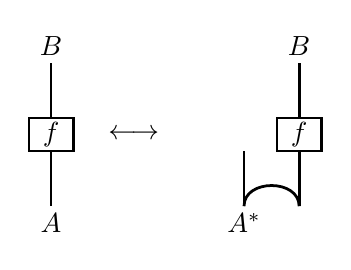
\begin{tikzpicture}[scale=0.7, line width=1pt]
  % LHS: process f : A -> B
  \draw (0,0) -- (0,1);
  \draw (-0.4,1) rectangle (0.4,1.6);
  \node at (0,1.3) {$f$};
  \draw (0,1.6) -- (0,2.6);
  \node at (0,-0.3) {$A$};
  \node at (0,2.9) {$B$};
  % arrow
  \node at (1.5,1.3) {$\longleftrightarrow$};
  % RHS: state of A^* tensor B via cup
  \draw (3.5,0) .. controls (3.5,0.5) and (4.5,0.5) .. (4.5,0);
  \draw (3.5,0) -- (3.5,1);
  \draw (4.5,0) -- (4.5,1);
  \draw (4.1,1) rectangle (4.9,1.6);
  \node at (4.5,1.3) {$f$};
  \draw (4.5,1.6) -- (4.5,2.6);
  \node at (3.5,-0.3) {$A^*$};
  \node at (4.5,2.9) {$B$};
\end{tikzpicture}
\end{center}

\subsection{Tensor decomposition and entanglement}

\begin{definition}[Pure separable state]
A state $\psi : I \to A \otimes B$ is \emph{pure separable} if it factors as $\psi = (\phi_A \otimes \phi_B) \circ \lambda_I^{-1}$ for some states $\phi_A : I \to A$ and $\phi_B : I \to B$.
\end{definition}

\begin{definition}[Pure entangled state]
A state of $A \otimes B$ is \emph{pure entangled} if it is not pure separable.
\end{definition}

\begin{proposition}
\label{prop:bell}
The state $\eta_A : I \to A^* \otimes A$ in a compact closed category is pure entangled whenever $A$ is not isomorphic to $I$.
\end{proposition}

\begin{proof}
Suppose $\eta_A = (\phi_{A^*} \otimes \phi_A) \circ \lambda_I^{-1}$. Composing with $\varepsilon_A$ yields, by the zig-zag identity, $\id_A = \phi_A \circ \varepsilon_A \circ (\phi_{A^*} \otimes \id_A)$, which factors $\id_A$ through $I$, forcing $A \cong I$.
\end{proof}

\begin{hook}[Hamiltonian hook $\mathsf{H2}$]
\label{hook:H2}
Define $\mathbf{Ham} \subseteq \Phys$ as the wide subcategory whose morphisms are unitaries generated by self-adjoint operators (Hamiltonians) under the exponential map $H \mapsto \exp(-i t H)$. $\mathbf{Ham}$ inherits the symmetric monoidal structure of $\Phys$ via $\exp(-i t (H_1 \otimes \id + \id \otimes H_2)) = \exp(-i t H_1) \otimes \exp(-i t H_2)$ when $[H_1 \otimes \id, \id \otimes H_2] = 0$. Law~II's adiabatic-deformation morphisms live in $\mathbf{Ham}$.
\end{hook}

\subsection{Worked diagrammatic identity: the snake equation}

We illustrate the diagrammatic style with the \emph{snake equation}, which is the diagrammatic content of the triangle identities of \cref{def:compact-closed}. Wires representing $A$ are drawn as upward-oriented strands; wires representing $A^*$ are drawn downward-oriented. The unit $\eta_A$ is a cup opening upward (a $\cup$-shape with $A^*$ on the left and $A$ on the right); the counit $\varepsilon_A$ is a cap closing downward.

The first triangle identity says that an $A$-strand which goes ``up, around the cap, down through the cup, and out the top'' is equal to the straight $A$-strand:
\[
(\id_A \otimes \varepsilon_A) \circ (\eta_A \otimes \id_A) = \id_A.
\]
Diagrammatically, this is the celebrated S-shape that straightens out into a vertical line:
\begin{center}
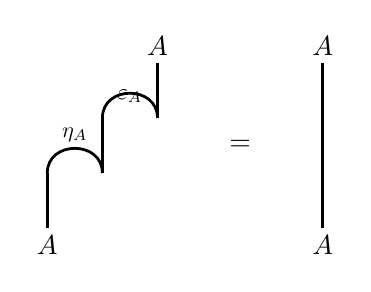
\begin{tikzpicture}[scale=0.7, line width=1pt]
  % LHS: snaking strand
  \draw (0,0) -- (0,1);
  \draw (0,1) .. controls (0,1.6) and (1,1.6) .. (1,1);
  \draw (1,1) -- (1,2);
  \draw (1,2) .. controls (1,2.6) and (2,2.6) .. (2,2);
  \draw (2,2) -- (2,3);
  \node at (0,-0.3) {$A$};
  \node at (2,3.3) {$A$};
  \node[scale=0.8] at (0.5,1.7) {$\eta_A$};
  \node[scale=0.8] at (1.5,2.4) {$\varepsilon_A$};
  % equality
  \node at (3.5,1.5) {$=$};
  % RHS: straight strand
  \draw (5,0) -- (5,3);
  \node at (5,-0.3) {$A$};
  \node at (5,3.3) {$A$};
\end{tikzpicture}
\end{center}
The second triangle identity is the mirror image with $A^*$. Both identities are required for the compact-closed structure: the first one ensures that an $A$-strand can be straightened, and the second one ensures the same for an $A^*$-strand. Together they say: in a compact closed category, ``slack can be pulled out of any wire,'' regardless of orientation. The whole framework of \cref{sec:matter-info-functor}---in particular \cref{thm:born} (Born rule) and the trace structure of \cref{hook:H7}---relies on \emph{both} triangle identities being available simultaneously, so we list them together as a single structural axiom rather than treating them separately.

This is the foundational identity used by the categorical formulation of quantum teleportation~\cite{abramskycoecke2004}: the teleportation protocol amounts to a diagrammatic snake straightening, in which the input wire of Alice's qubit is bent through a Bell pair (a $\eta$) and a Bell measurement (an $\varepsilon$), arriving at Bob with no further operation needed beyond a Pauli correction. Law~IV will use the same identity to derive the Ryu--Takayanagi-style entanglement-area formula in the HaPPY code~\cite{pastawski2015}.

\subsection{Frobenius algebras and bases}

\begin{definition}[Dagger Frobenius algebra]
A \emph{dagger Frobenius algebra} on $A$ in a dagger symmetric monoidal category is a tuple $(A, \mu, \eta, \delta, \varepsilon)$ with $\mu : A \otimes A \to A$, $\eta : I \to A$, $\delta = \mu^\dagger$, $\varepsilon = \eta^\dagger$, satisfying associativity, unitality, and the Frobenius law $(\id \otimes \mu) \circ (\delta \otimes \id) = \delta \circ \mu$.
\end{definition}

\begin{theorem}[Coecke--Pavlovic--Vicary~\cite{abramskycoecke2004}]
\label{thm:cpv}
Special commutative dagger Frobenius algebras in $\FHilb$ correspond bijectively to orthonormal bases.
\end{theorem}

\Cref{thm:cpv} is the categorical statement that ``measurement bases are algebraic data'' and not metric data: bases are characterised by the pure algebra of multiplication and copying.

\subsection{Adjunctions and quantisation}

A central organising device of the framework is the notion of adjunction. We recall the definition for completeness.

\begin{definition}[Adjunction]
\label{def:adjunction}
Given functors $F : \C \to \D$ and $G : \D \to \C$, we say $F$ is left adjoint to $G$ (written $F \dashv G$) if there is a bijection
\[
\Hom_\D(F(A), B) \;\cong\; \Hom_\C(A, G(B))
\]
natural in $A \in \C$ and $B \in \D$.
\end{definition}

Many physically meaningful functors come in adjoint pairs:
\begin{itemize}
\item The forgetful functor $U : \mathbf{Ham} \to \Phys$ has a left adjoint $\mathrm{Free} : \Phys \to \mathbf{Ham}$ assigning the free Hamiltonian (zero-coupling).
\item The inclusion $\Set \hookrightarrow \mathbf{Cat}$ has a left adjoint (free category on a set) and a right adjoint (codiscrete category).
\item Quantisation/dequantisation are conjecturally a Quillen adjoint pair between suitable categories of classical and quantum systems~\cite{lawvere1969}.
\end{itemize}

\begin{theorem}[Naturality of adjoints under $M$]
\label{thm:adjoint-naturality}
Let $F \dashv G$ be an adjunction in $\Phys$, and let $M : \Phys \to \Info$ be a strong monoidal dagger functor preserving finite limits and colimits. Then $M F \dashv M G$ is an adjunction in $\Info$, with unit and counit obtained by applying $M$ to those of the original adjunction.
\end{theorem}

\begin{proof}
The adjunction bijection $\Hom_\Phys(F(A), B) \cong \Hom_\Phys(A, G(B))$ is preserved by $M$ on hom-sets because $M$ is a functor, and naturality is preserved by functoriality of $M$ on the indexing variables. Limit/colimit preservation ensures that the universal property of unit/counit transfers.
\end{proof}

\Cref{thm:adjoint-naturality} is the formal statement that adjunctions in $\Phys$ are visible in $\Info$: phase-classifying adjunctions (Law~II) and Floquet-classifying adjunctions (Law~III) survive the matter--information passage.

\section{Sheaves and Topoi for Local Physics}
\label{sec:sheaves}

We now turn to the sheaf-theoretic refinement of the framework. The intuition is that physical observables are localised: a measurement is performed in a region of spacetime (or, more generally, a context). The collection of observables in each region forms a set or vector space, and these collections fit together in a structure-preserving way.

\subsection{Sites, presheaves, sheaves}

\begin{definition}[Site]
A \emph{site} is a small category $\C$ together with a Grothendieck topology $J$, i.e.\ for each $A \in \Ob(\C)$ a collection $J(A)$ of \emph{covering sieves}, satisfying the standard axioms (stability, transitivity, identity)~\cite{maclane1998}.
\end{definition}

\begin{definition}[Presheaf, sheaf]
A \emph{presheaf} on $\C$ is a functor $F : \C^\op \to \Set$. A \emph{sheaf} for the topology $J$ is a presheaf $F$ such that, for every covering sieve $S \in J(A)$, the natural map
\[
F(A) \longrightarrow \lim_{(B \to A) \in S} F(B)
\]
is a bijection.
\end{definition}

\begin{hook}[Sheaf hook $\mathsf{H4}$]
\label{hook:H4}
The site $(\C, J)$ controlling locality is a hook supplied by the physical context. Examples used in subsequent laws: (a) for Law~II, $\C$ is the poset of open subsets of a sample manifold and $J$ is the open-cover topology; (b) for Law~IV, $\C$ is a Boolean poset of measurement contexts and $J$ is the canonical topology of overlap.
\end{hook}

\subsection{Topoi and internal logic}

\begin{definition}[Grothendieck topos]
A \emph{Grothendieck topos} is a category equivalent to the category $\mathbf{Sh}(\C, J)$ of sheaves on a small site.
\end{definition}

\begin{theorem}[Giraud~\cite{maclane1998}]
\label{thm:giraud}
A category $\E$ is a Grothendieck topos if and only if it satisfies:
\begin{enumerate}
\item all small colimits exist and are universal;
\item coproducts are disjoint;
\item equivalence relations are effective;
\item there exists a set of generators.
\end{enumerate}
\end{theorem}

\begin{proposition}
Every Grothendieck topos $\E$ admits a \emph{subobject classifier} $\Omega \in \E$, characterised by the property that subobjects of any $A \in \E$ correspond bijectively to morphisms $A \to \Omega$. The internal language of $\E$ is intuitionistic higher-order logic.
\end{proposition}

\begin{hook}[Type-theoretic hook $\mathsf{H8}$]
\label{hook:H8}
The internal language $\mathcal{L}(\Info)$ of $\Info$, when $\Info$ has topos structure, supplies an executable encoding language. Subsequent laws use $\mathcal{L}(\Info)$ to write down phase classifiers, Floquet operators, and quantum codes as type-theoretic terms.
\end{hook}

\subsection{Lifting sheaves through \texorpdfstring{$M$}{M}}

\begin{theorem}[Sheaf-lifting through $M$, in the topos-theoretic regime]
\label{thm:sheaf-lifting}
\emph{Hypotheses.} Suppose that for the present application of the framework:
\begin{enumerate}
\item $\Phys$ is equivalent to the Grothendieck topos $\mathbf{Sh}(\C_\Phys, J_\Phys)$ of sheaves on a small site;
\item $\Info$ is equivalent to a Grothendieck topos $\mathbf{Sh}(\C_\Info, J_\Info)$;
\item $M : \Phys \to \Info$ is a strong monoidal dagger functor that, in addition, preserves finite limits and arbitrary small colimits.
\end{enumerate}
\emph{Conclusion.} Then $M$ arises as the inverse-image part $m^*$ of a geometric morphism of topoi, induced by a unique morphism of sites $m : (\C_\Info, J_\Info) \to (\C_\Phys, J_\Phys)$. That is, $M = m^* : \mathbf{Sh}(\C_\Phys, J_\Phys) \to \mathbf{Sh}(\C_\Info, J_\Info)$.

\emph{Scope.} \Cref{thm:sheaf-lifting} applies only when the hypotheses (1)--(3) hold; in particular it is not a structural fact about every matter--information functor, but only about those for which $\Phys$ and $\Info$ admit a topos-theoretic presentation. Laws~II and~IV use the theorem in regimes where these hypotheses are met.
\end{theorem}

\begin{proof}
The argument proceeds in three steps.

\smallskip\noindent
\emph{Step 1 (Geometric morphism from $M$).}\;
A geometric morphism $f : \E \to \mathcal{F}$ of Grothendieck topoi is by definition an adjunction $f^* \dashv f_*$ in which the left adjoint $f^*$ preserves finite limits. Conversely, given a finite-limit-preserving cocontinuous functor $M : \Phys \to \Info$, the special adjoint functor theorem (applicable because $\Phys$ is locally small with all small colimits) supplies a right adjoint $M_R : \Info \to \Phys$, and the pair $(M, M_R) = (m^*, m_*)$ is a geometric morphism $\Info \to \Phys$.

\emph{Step 2 (Site morphism inducing $m^*$).} By the Comparison Lemma~\cite{maclane1998}, a geometric morphism $\Info \to \Phys$ between sheaf topoi on small sites is determined by its restriction to the (full subcategories of) representable sheaves. The Yoneda embedding $y_\Phys : \C_\Phys \hookrightarrow \mathbf{Sh}(\C_\Phys, J_\Phys)$ is fully faithful, and similarly for $\Info$. Pulling $m^*$ back along $y_\Phys$ and using the universal property of sheafification gives a unique functor $m : \C_\Info \to \C_\Phys$ such that $m^* (y_\Phys(c)) = a(y_\Info(\overline{m}(c)))$ for some lift $\overline{m}$, where $a$ is sheafification. This $m$ is the site morphism in the statement, and the direction is forced: the inverse-image part of a geometric morphism between sheaf topoi corresponds at the site level to a functor running in the \emph{opposite} direction.

\emph{Step 3 (Uniqueness).} Any other site morphism $m'$ inducing the same $m^*$ would give the same restriction to representables (by Yoneda), hence agree with $m$. Uniqueness follows.
\end{proof}

\Cref{thm:sheaf-lifting} is the formal statement that local-observable structure is preserved by $M$. The geometric-morphism formulation makes explicit that $M$ behaves like the topos-theoretic ``pullback of observables along a generalised continuous map between informational and physical sites.''

\section{Operadic Composition Laws}
\label{sec:operads}

Operads control multi-input operations and are essential for the algebraic description of observables in QFT.

\subsection{Operads and their algebras}

\begin{definition}[Operad in $\Set$]
An \emph{operad} $O$ is a sequence of sets $\{O(n)\}_{n \geq 0}$ together with:
\begin{enumerate}
\item composition maps $\gamma : O(n) \times O(k_1) \times \cdots \times O(k_n) \to O(k_1 + \cdots + k_n)$;
\item a unit $1 \in O(1)$;
\item a right action of $\Sigma_n$ on $O(n)$;
\end{enumerate}
satisfying associativity, unitality, and equivariance.
\end{definition}

\begin{definition}[Algebra over an operad]
An \emph{algebra} over $O$ in a symmetric monoidal category $\C$ is an object $A \in \C$ together with maps $O(n) \otimes A^{\otimes n} \to A$ that respect $\gamma$, the unit, and the symmetric action.
\end{definition}

\begin{example}[$E_n$ operads]
\label{ex:En}
The little $n$-disks operad $E_n$ has $E_n(k)$ the space of $k$ disjoint $n$-disks inside the unit $n$-disk. Algebras over $E_n$ in topological spaces are $n$-fold loop spaces (May's recognition principle). Algebras over $E_\infty := \mathrm{colim}_n E_n$ are commutative algebras up to coherent homotopy.
\end{example}

\begin{hook}[Operadic hook $\mathsf{H5}$]
\label{hook:H5}
For each $n$, an $E_n$-algebra structure on a designated object of $\Info$ encodes the multi-region multiplication of observables at codimension $n$. Law~IV uses this hook to encode the factorisation algebra of a local QFT~\cite{costello2017}.
\end{hook}

\subsection{Factorisation algebras}

\begin{definition}[Prefactorisation algebra]
A \emph{prefactorisation algebra} on a manifold $M$, valued in a symmetric monoidal category $\C$, assigns to each open $U \subseteq M$ an object $F(U) \in \C$, and to each pairwise disjoint inclusion $U_1 \sqcup \cdots \sqcup U_n \hookrightarrow V$ a morphism
\[
F(U_1) \otimes \cdots \otimes F(U_n) \to F(V),
\]
satisfying associativity and unitality.
\end{definition}

\begin{definition}[Factorisation algebra~\cite{costello2017}]
A prefactorisation algebra is a \emph{factorisation algebra} if it satisfies a homotopy-coherent local-to-global condition for Weiss covers (covers stable under finite intersections).
\end{definition}

The relation to operads: the local structure of a factorisation algebra at a point is an $E_n$-algebra, where $n = \dim M$.

\section{Type-Theoretic Encoding}
\label{sec:type-theory}

We close the categorical setup with the type-theoretic encoding, which is what makes Law~I directly executable in a programming language such as Haskell.

\subsection{Curry--Howard--Lambek}

\begin{theorem}[Curry--Howard--Lambek correspondence~\cite{lambekscott1986}]
\label{thm:chl}
There is a triangle of equivalences:
\begin{itemize}
\item Cartesian closed categories $\;\leftrightarrow\;$ simply typed $\lambda$-calculi $\;\leftrightarrow\;$ intuitionistic propositional logics.
\item Symmetric monoidal closed categories $\;\leftrightarrow\;$ linear $\lambda$-calculi $\;\leftrightarrow\;$ intuitionistic linear logic.
\item Compact closed categories with dagger $\;\leftrightarrow\;$ quantum $\lambda$-calculi $\;\leftrightarrow\;$ multiplicative linear logic with involutive negation.
\end{itemize}
\end{theorem}

For our purposes, the third row is the relevant one: a quantum process is a term of a linear $\lambda$-calculus with involution, equivalently a morphism in a dagger compact closed category.

\subsection{Linear types and quantum resources}

The no-cloning theorem asserts that no quantum channel $\mathrm{copy} : H \to H \otimes H$ exists for non-trivial $H$. Linearly, this is the statement that the type $A$ has no canonical map $A \to A \otimes A$. Linear type systems encode this by forbidding contraction (variable duplication).

\subsection{Haskell encoding}

We encode the categorical hierarchy in Haskell as a sequence of type classes (the full code is supplied in the companion package, \cref{sec:examples}):

\begin{verbatim}
class Category cat where
  cid    :: cat a a
  ccomp  :: cat b c -> cat a b -> cat a c

class Category cat => MonoidalCategory cat where
  type Unit cat
  -- The Haskell pair type (,) realises the monoidal product on
  -- objects. We rely on Haskell's product-type constructor as
  -- a concrete witness of the abstract tensor.
  tensor :: cat a b -> cat c d -> cat (a, c) (b, d)

class Functor1 f where
  fmap1 :: (a -> b) -> f a -> f b

class (Category src, Category tgt) => CFunctor src tgt f where
  -- The dummy method fobj witnesses the type-level object map a -> f a.
  -- See note below regarding phantom encoding.
  fobj :: f a -> ()
  fmor :: src a b -> tgt (f a) (f b)
\end{verbatim}

\paragraph{Concretely realising the monoidal product.} The type signature
\begin{center}\small
\verb|tensor :: cat a b -> cat c d -> cat (a,c) (b,d)|
\end{center}
uses Haskell's built-in product type \verb|(,)| to realise the monoidal product at the type level. This is a deliberate choice: in our concrete instance \verb|Fn| (Hask + total functions), the categorical product \emph{is} the Haskell pair, so \verb|(a,c)| really is the image of $a \otimes c$ on objects. For other instances (e.g.\ a future linearly-typed \verb|LinFn|) one would replace the pair with a dedicated linear-tensor type constructor, and the corresponding tensor signature would map a pair of morphisms over $a, b$ and $c, d$ to a morphism over the tensors $a \otimes c$ and $b \otimes d$. The pair-based version above is the cartesian special case.

A note on the encoding of the object component. In Haskell, the object mapping of a functor cannot be made first-class without dependent types: objects of $\Phys$ would need to be Haskell types, and a functor's object map would need to be a type-level function. We follow the standard pragmatic idiom: the type parameter \verb|f a| carries the object information at the type level (so \verb|f a| \emph{is} the image of object \verb|a| under the functor), and the dummy method \verb|fobj :: f a -> ()| merely witnesses this assignment for the type-class machinery. Readers steeped in pure category theory should read \verb|fobj| as a phantom artefact of Haskell's stratification of types and values; the genuine ``object component'' of the functor is the type-level assignment $a \mapsto f\,a$.

\paragraph{Scope and limitations of the Haskell encoding.} The encoding above captures the \emph{categorical skeleton} of Law~I: identity, composition, the monoidal product, and the strong-monoidal functor signature. It does \emph{not} capture two structural ingredients of \cref{def:matter-info}:
\begin{enumerate}
\item \emph{Linearity.} Standard Haskell types support unrestricted contraction and weakening (variables can be duplicated and discarded), which is incompatible with the no-cloning and no-deletion theorems of quantum mechanics. Concretely: a Haskell function \texttt{a -> b} can in general duplicate or discard its argument, but if \texttt{a} and \texttt{b} are intended to model quantum states then this would correspond to a copying or deleting channel, which is not a structure-preserving morphism in $\FHilb$. A faithful encoding therefore requires the GHC \texttt{LinearTypes} extension (GHC 9.0+) or a dedicated linear-type framework such as Proto-Quipper-M~\cite{fukishidaselinger2020}.
\item \emph{Dagger.} The dagger functor $\dagger$ is involutive and identity-on-objects. Encoding it requires either a wrapper type (\verb|Dagger cat a b| as a pair of forward and backward morphisms) or a more sophisticated approach using inverse semicategories. Our \verb|Dagger|-\verb|Category| type class supplies the signature but does not enforce involutivity at the type level.
\end{enumerate}
Consequently, the executable-encoding hook $\mathsf{H8}$ is realised at the level of the categorical skeleton; full realisation, including linearity and dagger involution, is one of the open problems we list in \cref{sec:open-problems}. The property test suite (in-house, QuickCheck-style; see the companion package) verifies the category and monoidal laws on the present skeleton.

\begin{hook}[Dagger hook $\mathsf{H6}$, Floquet hook $\mathsf{H3}$]
The dagger hook $\mathsf{H6}$ is supplied by an additional type class \texttt{DaggerCategory} with method \texttt{dagger :: cat a b -> cat b a}; the Floquet hook $\mathsf{H3}$ is supplied by a one-object category \texttt{newtype B Z = B Integer} together with a functor \texttt{B Z -> Aut Phys}. Both are realised in the companion code.
\end{hook}

\section{Worked Examples}
\label{sec:examples}

We now exhibit four concrete examples of the framework, drawn from the four corners of the Rosetta Stone~\cite{baezstay2009}.

\subsection{Example 1: \texorpdfstring{$\FHilb$}{FHilb} as physics + information}

Let $\Phys = \Info = \FHilb$, and $M = \id$. This is the trivial instance, but it already exhibits all eight composition hooks:
\begin{itemize}
\item $\mathsf{H1}$: a unitary group action $G \to U(H)$ for each object $H$.
\item $\mathsf{H2}$: $\mathbf{Ham}$ is the wide subcategory of $\FHilb$ with self-adjoint generators.
\item $\mathsf{H3}$: a Floquet drive is a 1-parameter family of unitaries $U(t+T) = U(t)$.
\item $\mathsf{H4}$: the topology on the spectrum of an observable defines the sheaf hook.
\item $\mathsf{H5}$: the standard $E_n$-algebra of vacuum expectation values.
\item $\mathsf{H6}$: $\dagger$ is the Hilbert-space adjoint.
\item $\mathsf{H7}$: $H^* = \overline{H}$, $\eta$ and $\varepsilon$ are Bell pairing.
\item $\mathsf{H8}$: the internal language is multiplicative linear logic.
\end{itemize}

\subsection{Example 2: \texorpdfstring{$(1{+}1)$D}{(1+1)D} TQFT}

Let $\Phys = \Cob_2$ and $\Info = \FHilb$. By Atiyah's axioms~\cite{atiyah1988}, $M : \Cob_2 \to \FHilb$ is a symmetric monoidal functor. By the classification of $(1+1)$D TQFTs:

\begin{theorem}[$(1+1)$D TQFT classification~\cite{atiyah1988,baezstay2009}]
\label{thm:11d-tqft}
$(1+1)$D TQFTs are in bijection with finite-dimensional commutative Frobenius algebras: $M$ is determined by $A := M(S^1)$, which inherits a commutative Frobenius algebra structure from the pair-of-pants and cap cobordisms.
\end{theorem}

\begin{proof}[Proof sketch]
The pair-of-pants cobordism $S^1 \sqcup S^1 \to S^1$ gives multiplication $\mu : A \otimes A \to A$; the reversed pair-of-pants gives comultiplication; the cap and cocap give unit and counit. Frobenius and commutativity follow from the topological identities on the bordisms.
\end{proof}

\subsection{Example 3: presheaves on a poset}

Let $\C$ be a finite poset (e.g.\ a Boolean lattice of measurement contexts) and let $\Info = \mathbf{PSh}(\C) = \mathbf{Sh}(\C, J_{\mathrm{trivial}})$. The Yoneda embedding $y : \C \to \mathbf{PSh}(\C)$ exhibits every object of $\C$ as a representable presheaf. The matter--information functor is then a Grothendieck construction: given a fibration of categories over $\C$, take fibrewise data.

\subsection{Example 4: little disks operad on a Hilbert space}

Let $A \in \FHilb$ be a vector space carrying an $E_2$-algebra structure (e.g.\ a vertex operator algebra for $\mathrm{Vir}_c$). The operadic hook $\mathsf{H5}$ assigns each pair of disjoint disks $D_1, D_2 \subset D$ a multiplication $A \otimes A \to A$ depending continuously on the configuration. This is the seed of Law~IV's holographic factorisation algebras.

\subsection{Example 5: Lawvere and linear theories}

This example highlights the bits/qubits asymmetry through Lawvere theories and their symmetric monoidal generalisation. A \emph{Lawvere theory}~\cite{lawvere1963} is a small category $T$ with finite products, equipped with a distinguished object $X$ such that every object is isomorphic to a finite power $X^n$. A \emph{model} of $T$ in a category $\C$ with finite products is a finite-product-preserving functor $T \to \C$.

For classical bits, take $T_{\mathrm{Bit}}$ to be the Lawvere theory generated by morphisms
\[
\mathrm{copy} : X \to X \times X,\qquad \mathrm{xor} : X \times X \to X,\qquad 0, 1 : * \to X,
\]
modulo the axioms of Boolean algebra. Models of $T_{\mathrm{Bit}}$ in $\Set$ are precisely Boolean algebras: a model assigns to $X$ an underlying set, and to each generator a function compatible with the Boolean axioms.

To extend this picture to quantum bits, one cannot work in a category with finite products, because the diagonal $\Delta_X : X \to X \times X$ (the universal copying map associated with the categorical product) does not correspond to a quantum channel---its image under any candidate functor $T_{\mathrm{Bit}} \to \FHilb$ would be a $\mathbb{C}$-linear copying map $\mathbb{C}^2 \to \mathbb{C}^2 \otimes \mathbb{C}^2$, which is forbidden by no-cloning.

The correct replacement is a \emph{symmetric monoidal Lawvere theory}, also called a \emph{PROP} (\emph{products and permutations category}) in the literature: a small symmetric strict monoidal category whose objects are the natural numbers under addition, generated by a chosen set of morphisms modulo relations. We define:

\begin{definition}[Linear Lawvere theory]
\label{def:linear-lawvere}
A \emph{linear Lawvere theory}, or \emph{linear PROP}, is a small symmetric strict monoidal category $T_\mathrm{lin}$ whose monoid of objects is $(\mathbb{N}, +, 0)$, generated by a chosen set of morphisms together with a chosen set of relations among them. A \emph{model} of $T_\mathrm{lin}$ in a symmetric monoidal category $\C$ is a strong symmetric monoidal functor $T_\mathrm{lin} \to \C$.
\end{definition}

Crucially, a linear Lawvere theory has no \emph{a priori} diagonal: the tensor $X \otimes X$ is not a categorical product, and there is no canonical morphism $X \to X \otimes X$. To define a copying-style operation one must adjoin a generating morphism, and this adjunction is where the quantum/classical distinction lives: the linear theory $T_{\mathrm{Qubit}}$ generated only by Hadamard, phase, and CNOT (without a copy generator) embeds faithfully into $\FHilb$, whereas its classical projection (replacing CNOT with $\mathrm{copy}$) does not.

This is the categorical statement of the bits/qubits asymmetry:
\begin{itemize}
\item Classical models live in cartesian categories ($\Set$, $\mathbf{Top}$, etc.) and admit canonical diagonals.
\item Quantum models live in symmetric monoidal (non-cartesian) categories and have no canonical diagonals; the absence of $\mathrm{copy}$ is enforced at the categorical level.
\end{itemize}

The matter--information functor $M : \Phys \to \Info$, when both $\Phys$ and $\Info$ are quantum-style symmetric monoidal categories, automatically respects this absence; when $\Info$ is a classical environment (e.g.\ $\Info = \Set$), the functor cannot be strong monoidal in the symmetric monoidal sense, and one must pass through a \emph{decoherence} structure (a commutative dagger Frobenius algebra) to mediate the transition. This example is paradigmatic for how the matter--information correspondence differs from a naive set-valued semantics.

\subsection{Lifting points for downstream laws}

We collect the lifting points that Laws~II--IV inherit from Law~I:

\begin{center}
\begin{tabular}{lll}
\toprule
Hook & Used by & Realisation in series \\
\midrule
$\mathsf{H1}$ Symmetry & II, III & $G$-action on Hamiltonians; Floquet $\mathbb{Z}$-action \\
$\mathsf{H2}$ Hamiltonian & II, III & Gapped phase classifier; adiabatic deformations \\
$\mathsf{H3}$ Floquet & III & $B\mathbb{Z}$-functors and natural transformations \\
$\mathsf{H4}$ Sheaf & II, IV & Local order parameters; CFT data \\
$\mathsf{H5}$ Operadic & IV & Factorisation algebras; vertex operators \\
$\mathsf{H6}$ Dagger & III, IV & Unitarity; QEC code structure \\
$\mathsf{H7}$ Compact & IV & Trace, partial trace; Ryu--Takayanagi \\
$\mathsf{H8}$ Type-theory & II, III, IV & Executable encodings \\
\bottomrule
\end{tabular}
\end{center}

\section{Open Problems}
\label{sec:open-problems}

We list four open problems that the foundational layer (Law~I) leaves to future work, in roughly increasing order of ambition:

\begin{enumerate}
\item \textbf{Renormalisation as a categorical structure.} Atiyah's TQFT axioms work for finite-dimensional models. A categorical axiomatisation of QFT that handles infinite-dimensional Hilbert spaces and renormalisation, perhaps via Costello--Gwilliam factorisation algebras, remains an open problem of foundational interest~\cite{costello2017}.
\item \textbf{Linear dependent type theory and measurement.} A type theory with linear dependent types that is computationally tractable and sound for categorical quantum mechanics with measurements would close the type-theoretic hook $\mathsf{H8}$ at the level needed for Laws~III--IV~\cite{fukishidaselinger2020}.
\item \textbf{Cohesive HoTT vs.\ factorisation algebras.} The relationship between Schreiber--Shulman's cohesive HoTT~\cite{schreibershulman2014} and the factorisation-algebra approach to QFT~\cite{costello2017} for flat spacetimes is conjectured but not proven equivalent.
\item \textbf{Born rule beyond Gleason.} A purely categorical characterisation of the Born rule, beyond the existing assumption of compact closure with dagger and beyond Gleason's theorem on lattices of projections, remains a foundational target~\cite{abramskycoecke2004}.
\end{enumerate}

\section{Discussion}
\label{sec:discussion}

\subsection{What Law~I does and does not claim}

Law~I claims a structural fact: \emph{if} matter and information are organised as objects of suitably structured symmetric monoidal categories, \emph{then} their relation is forced to be a strong monoidal dagger functor satisfying the conditions of \cref{def:matter-info}. The hooks $\mathsf{H1}$--$\mathsf{H8}$ are slots; they are not filled by Law~I.

Law~I does \emph{not} claim:
\begin{itemize}
\item that the categorical formulation is unique. There are alternative formulations (e.g.\ algebraic QFT in the Haag--Kastler sense, or operator algebraic settings).
\item that all of physics is captured. We address only the matter--information correspondence layer; dynamics, gravity, and renormalisation are addressed in the subsequent laws.
\item that the framework is complete. Many of the open problems in \cref{sec:open-problems} are precisely about completion.
\end{itemize}

\subsection{Comparison with related programmes}

The framework here is closest in spirit to the categorical quantum mechanics programme of Abramsky--Coecke~\cite{abramskycoecke2004} and the higher-categorical TQFT programme of Lurie~\cite{lurie2009}. The novelty is the explicit declaration of composition hooks: rather than presenting a self-contained mathematical edifice, we present a structured interface designed to be filled by downstream laws. This methodological choice is what makes the programme \emph{modular} rather than unified.

\subsection{Categorical entropy and the bridge to information}

A natural objection to the present formulation is that it does not visibly contain entropy or any quantitative measure of information. We respond by recalling the categorical characterisation of Shannon entropy due to Baez--Fritz--Leinster: Shannon entropy is the unique (up to scale) functor $H : \mathbf{FinProb} \to [0,\infty)$ satisfying functoriality, the chain rule, and continuity, where $\mathbf{FinProb}$ is the category of finite probability spaces and measure-preserving maps. This characterisation lifts to $\Info$ provided $\Info$ contains a sub-monoidal category equivalent to $\mathbf{FinProb}$.

\begin{remark}[Information measures as functors]
The slogan ``information is functorial'' is realised concretely: every reasonable information-theoretic quantity (Shannon, R\'enyi-$\alpha$, von Neumann, conditional, mutual, relative) admits a categorical characterisation. Law~IV uses these characterisations to reduce holographic entanglement-entropy formulas to functorial identities.
\end{remark}

\subsection{Connection to the cobordism hypothesis as ``representability''}

\Cref{thm:cobordism} (Cobordism Hypothesis) plays a methodologically distinctive role in our framework: it is a \emph{representability theorem}. It says that every symmetric monoidal $(\infty,n)$-functor out of $\Bord_n^{\mathrm{fr}}$ is represented by its value at the point. We invoke this representability to argue that the matter--information functor $M$ is determined by very little data---in the cobordism case, by the single object $M(\mathrm{pt})$, which must be fully dualisable.

This has an immediate methodological corollary: \emph{when working with a fixed category $\Phys$ that admits a presentation as a free symmetric monoidal $(\infty,n)$-category with duals, the matter--information functor is fixed by the specification of a single fully-dualisable object in $\Info$}. Downstream laws use this principle to constrain their constructions: Law~II's phase classifier, Law~III's Floquet operator, and Law~IV's holographic code each amount to a choice of fully-dualisable object satisfying additional constraints.

\subsection{Modular composition, not unification}

Throughout, we have insisted on modular language. The four-law programme is not a unified theory; it is a \emph{stack of layers}, each layer self-standing, with composition controlled by functors and natural transformations. The reader who finds, say, Law~III's Floquet category problematic can in principle replace it with another category satisfying the hook $\mathsf{H3}$, and the rest of the programme continues to apply. This is the engineering virtue of the modular approach.

\section{Conclusion}
\label{sec:conclusion}

We have introduced Law~I of a four-paper modular programme: the categorical foundations for matter--information correspondence. The contributions are:
\begin{enumerate}
\item A precise definition of the matter--information functor $M : \Phys \to \Info$ as a strong monoidal dagger functor.
\item Three structural results: generation of $M$ from a presentation (\cref{thm:generation}), a Born-rule type formula from compact closure (\cref{thm:born}), and sheaf lifting through $M$ (\cref{thm:sheaf-lifting}).
\item Eight composition hooks $\mathsf{H1}$--$\mathsf{H8}$ that downstream laws (II--IV) plug into, with explicit signature and intended semantics.
\item A Haskell encoding of the categorical skeleton with QuickCheck property tests for the category and monoidal laws.
\item Worked examples drawn from $\FHilb$, the cobordism category, presheaves on a poset, and the little-disks operad.
\end{enumerate}

The next paper in the series, Law~II (\emph{Phase-bound Matter}), uses these hooks (particularly $\mathsf{H1}, \mathsf{H2}, \mathsf{H4}, \mathsf{H8}$) to classify thermodynamic and topological phases as functors over symmetry-group categories.

\subsection{Compositional roadmap}

The four-paper modular series composes its laws in the following order:
\begin{enumerate}
\item \textbf{Law~I (this paper):} Categorical primitives. Output: hooks $\mathsf{H1}$--$\mathsf{H8}$ and a matter--information functor $M : \Phys \to \Info$.
\item \textbf{Law~II (Phase-bound Matter):} Plug $\mathsf{H1}, \mathsf{H2}, \mathsf{H4}, \mathsf{H8}$. Output: a functor $\mathrm{Phase} : B G \to \mathbf{Ham} / \!\sim_{\mathrm{adiabatic}}$ classifying gapped phases.
\item \textbf{Law~III (Frequency-modulated Processes):} Plug $\mathsf{H3}, \mathsf{H6}$. Output: a Floquet functor $F : B \mathbb{Z} \to \Phys$ and its natural-transformation classifications. Composes with Law~II to produce non-equilibrium phase classifiers.
\item \textbf{Law~IV (Information-bearing Structures):} Plug $\mathsf{H5}, \mathsf{H7}$. Output: a holographic code (HaPPY-type) realised as a fully-dualisable object whose tensor-network geometry computes Ryu--Takayanagi-style entanglement entropies.
\end{enumerate}
The synthesis paper then exhibits the composite of all four laws, in which each layer's hook is realised by the layer above. The composition is not unique---different physical systems give different fillings of the same hooks---but the \emph{type} of the composite is fixed by Law~I.

\subsection{What a reader of Law~I should take away}

Three concrete takeaways are intended:
\begin{itemize}
\item The matter--information correspondence is the \emph{type} of a structure-preserving functor between two symmetric monoidal dagger categories. Anything compatible with this type is a candidate matter--information correspondence.
\item Eight composition hooks give precise interfaces for downstream layers. A reader implementing a new layer should ask: which hooks does it consume, and which does it leave untouched?
\item The framework is \emph{modular}, not unified. Replacing any single layer with a different filling of its hook leaves the rest of the framework intact, because the only contract between layers is the typed hook signature.
\end{itemize}

\begin{thebibliography}{99}

\bibitem{atiyah1988}
M.~Atiyah,
\emph{Topological quantum field theories},
Publications Math\'ematiques de l'IH\'ES \textbf{68} (1988) 175--186.

\bibitem{baezdolan1995}
J.~C.~Baez and J.~Dolan,
\emph{Higher-dimensional algebra and topological quantum field theory},
J.\ Math.\ Phys.\ \textbf{36} (1995) 6073--6105.

\bibitem{baezstay2009}
J.~C.~Baez and M.~Stay,
\emph{Physics, topology, logic and computation: a Rosetta Stone},
in: \emph{New Structures for Physics}, Lecture Notes in Physics \textbf{813}, Springer (2011), pp.~95--172; arXiv:0903.0340.

\bibitem{abramskycoecke2004}
S.~Abramsky and B.~Coecke,
\emph{A categorical semantics of quantum protocols},
in: Proc.\ 19th IEEE Symposium on Logic in Computer Science (2004), pp.~415--425; extended as \emph{Categorical quantum mechanics}, in: \emph{Handbook of Quantum Logic and Quantum Structures}, Elsevier (2008), pp.~261--323.

\bibitem{lurie2009}
J.~Lurie,
\emph{Higher Topos Theory},
Annals of Mathematics Studies \textbf{170}, Princeton University Press, Princeton, NJ (2009); arXiv:math/0608040.

\bibitem{schreibershulman2014}
U.~Schreiber and M.~Shulman,
\emph{Quantum gauge field theory in cohesive homotopy type theory},
Electronic Proceedings in Theoretical Computer Science \textbf{158} (2014) 109--126; arXiv:1408.0054.

\bibitem{lawvere1963}
F.~W.~Lawvere,
\emph{Functorial semantics of algebraic theories},
Proc.\ Natl.\ Acad.\ Sci.\ USA \textbf{50} (1963) 869--872; reprinted in Reprints in Theory and Applications of Categories \textbf{5} (2004).

\bibitem{lawvere1969}
F.~W.~Lawvere,
\emph{Adjointness in foundations},
Dialectica \textbf{23} (1969) 281--296.

\bibitem{maclane1998}
S.~Mac~Lane,
\emph{Categories for the Working Mathematician},
2nd ed., Graduate Texts in Mathematics \textbf{5}, Springer, New York (1998).

\bibitem{joyalstreet1991}
A.~Joyal and R.~Street,
\emph{The geometry of tensor calculus I},
Adv.\ Math.\ \textbf{88} (1991) 55--112.

\bibitem{costello2017}
K.~Costello and O.~Gwilliam,
\emph{Factorization Algebras in Quantum Field Theory}, Vol.~1,
New Mathematical Monographs \textbf{31}, Cambridge University Press, Cambridge (2017).

\bibitem{lambekscott1986}
J.~Lambek and P.~J.~Scott,
\emph{Introduction to Higher Order Categorical Logic},
Cambridge Studies in Advanced Mathematics \textbf{7}, Cambridge University Press, Cambridge (1986).

\bibitem{fukishidaselinger2020}
P.~Fu, K.~Kishida, and P.~Selinger,
\emph{Linear dependent type theory for quantum programming languages},
in: Proc.\ 35th Annual ACM/IEEE Symposium on Logic in Computer Science (LICS) 2020, pp.~440--453; arXiv:2004.13472.

\bibitem{kitaev2003}
A.~Yu.~Kitaev,
\emph{Fault-tolerant quantum computation by anyons},
Ann.\ Phys.\ \textbf{303} (2003) 2--30; arXiv:quant-ph/9707021.

\bibitem{pastawski2015}
F.~Pastawski, B.~Yoshida, D.~Harlow, and J.~Preskill,
\emph{Holographic quantum error-correcting codes: toy models for the bulk/boundary correspondence},
J.\ High Energy Phys.\ \textbf{2015} (2015) 149; arXiv:1503.06237.

\bibitem{ryu2006}
S.~Ryu and T.~Takayanagi,
\emph{Holographic derivation of entanglement entropy from AdS/CFT},
Phys.\ Rev.\ Lett.\ \textbf{96} (2006) 181602; arXiv:hep-th/0603001.

\bibitem{amari2016}
S.-I.~Amari,
\emph{Information Geometry and Its Applications},
Applied Mathematical Sciences \textbf{194}, Springer, Tokyo (2016).

\end{thebibliography}

\end{document}
